\section{The update functions}
The update functions are given as:

\begin{align}
    \tilde{I}^{m+\frac{1}{2}}_{n+\frac{1}{2}} = \tilde{I}^{m-\frac{1}{2}}_{n+\frac{1}{2}} + \alpha\left(V^{m}_{n} - V^{m}_{n+1}\right) \label{update}, \quad\quad
    V^{m+1}_n = V^{m}_{n} + \alpha\left(\tilde{I}^{m+\frac{1}{2}}_{n-\frac{1}{2}}-\tilde{I}^{m+\frac{1}{2}}_{n+\frac{1}{2}}\right),  
    \end{align}
    
where
\begin{equation}
\alpha \triangleq \frac{v\Delta t}{\Delta z}
    \label{alpha}
\end{equation}

is the dimensionless Courant factor and
\begin{equation}
    \tilde{I}^{m+\frac{1}{2}}_{n+\frac{1}{2}} = I^{m+\frac{1}{2}}_{n+\frac{1}{2}}R_c
    \label{Itil}
\end{equation}
is the rescaled current.

At the boundaries the update function for $V$ takes another form.
\begin{itemize}
    \item At $z = 0$\\
    The voltage update function is given as:
    \begin{equation}
        V^{m+1}_{0} = V^{m}_{0} + \frac{2\Delta t}{C\Delta z}\left(I^{m+\frac{1}{2}}_{g} - I^{m+\frac{1}{2}}_{\frac{1}{2}}\right),
        \label{BC1}
    \end{equation}
    with 
    \begin{equation}
        I^{m+\frac{1}{2}}_{g} = \frac{E^{m+\frac{1}{2}}_{g}}{R_{g}}-\frac{V^{m}_{0}+V^{m+1}_{0}}{2R_g}.
        \label{Ig}
    \end{equation}
    Subsituting (\ref{Ig}) in (\ref{BC1}) and ussing (\ref{alpha}), the two relations $v=\frac{1}{\sqrt{LC}}$ and $R_c=\sqrt{\frac{L}{C}}$ and the new defined constant $\tilde{R}_{g} = \frac{R_c}{R_g}$ yields, 
    after some rearrangements:
    \begin{equation}
        V^{m+1}_{0} = C_{1}V^{m}_{0} + C_{2}\left(E^{m+\frac{1}{2}}_{g}\tilde{R}_{g} - \tilde{I}^{m+\frac{1}{2}}_{\frac{1}{2}}\right)
    \end{equation}
    where
    \begin{align}
        C_{1} & = \frac{1-\alpha\tilde{R}_{g}}{1+\alpha\tilde{R}_{g}},\\
        C_{2} & = \frac{2\alpha}{1+\alpha\tilde{R}_{g}},
    \end{align}
    are two dimensionless constants.
    \item At $z = l$\\
    
    \begin{center}
    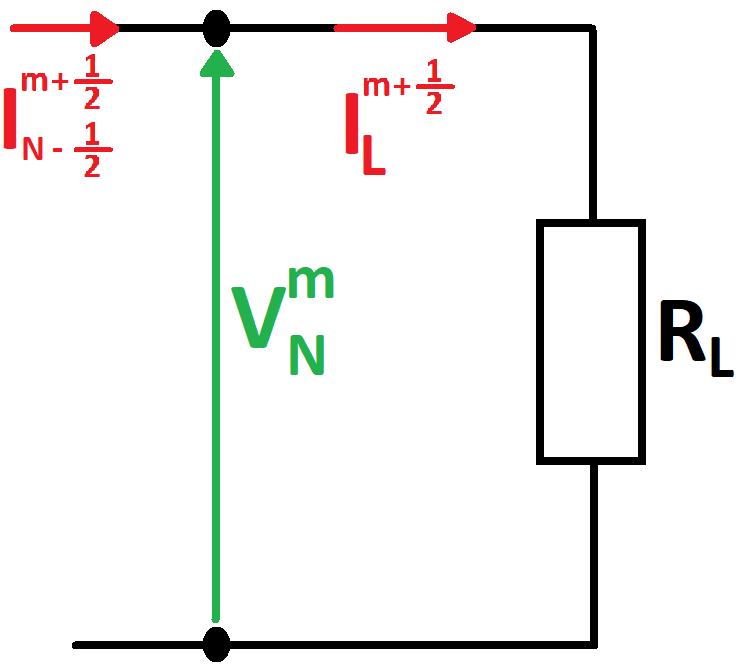
\includegraphics[scale=0.25]{BC2}
    \end{center}

    The voltage update function becomes:
    \begin{equation}
        V^{m+1}_{N} = V^{m}_{N} + \frac{2\Delta t}{C\Delta z}\left(I^{m+\frac{1}{2}}_{N-\frac{1}{2}} - I^{m+\frac{1}{2}}_{L}\right)
        \label{BC2}
    \end{equation}
    Kirchoff's voltage law in discretized form states that
    \begin{align}
        I^{m+\frac{1}{2}}_{L} & = \frac{V^{m+\frac{1}{2}}_{N}}{R_{L}}\\
        & = \frac{V^{m}_{N}+V^{m+1}_{N}}{2R_{L}}
        \label{IL}
    \end{align}
    Subsituting (\ref{IL}) in (\ref{BC2}) and using the same relations as for $z=0$ and the new defined constant $\tilde{R}_{L} = \frac{R_c}{R_L}$ yields, 
    after some rearrangements:
    \begin{equation}
        V^{m+1}_{N} = C_{3}V^{m}_N + C_{4}\tilde{I}^{m+\frac{1}{2}}_{N-\frac{1}{2}},
    \end{equation}
    where
    \begin{align}
        C_{3} & = \frac{1-\alpha\tilde{R}_{L}}{1+\alpha\tilde{R}_{L}},\\
        C_{4} & = \frac{2\alpha}{1+\alpha\tilde{R}_{L}},
    \end{align}
    are two dimensionless constants.

    Now if there would be a capacitor added to the load the following situation will occur
    
    \begin{center}
    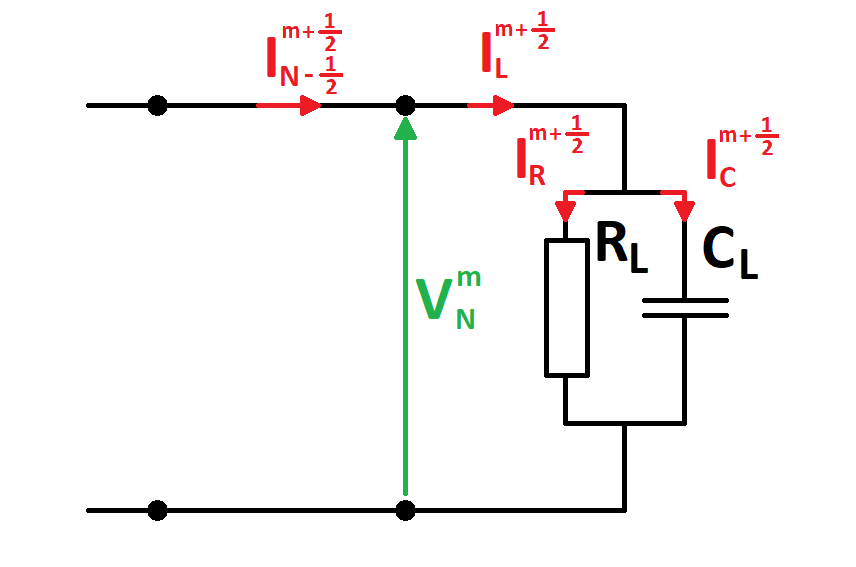
\includegraphics[scale=0.35]{BC2_cap}
    \end{center}
    
    Kirchoff's current law states that
    \begin{equation}
        I^{m+\frac{1}{2}}_{L} = I^{m+\frac{1}{2}}_{R} + I^{m+\frac{1}{2}}_{C}.
        \label{IL2}
    \end{equation}
    Using Kirchoff's voltage law at the resistor gives
    \begin{align}
        I^{m+\frac{1}{2}}_{R} & = \frac{V^{m+\frac{1}{2}}_{N}}{R_{L}}\\
        & = \frac{V^{m}_{N}+V^{m+1}_{N}}{2R_{L}}
        \label{IR}
    \end{align}
    The relation between the current and the voltage at the capitor is given as
    \begin{equation}
        \hat{i} = -C\frac{\partial \hat{v}}{\partial t}.
    \end{equation}
    For a first order FDM this turns into
    \begin{equation}
        I^{m+\frac{1}{2}}_{R} = -C_{L}\frac{V^{m+1}_{N} - V^{m}_{N}}{\Delta t}.
        \label{IC}
    \end{equation}
    Substituting (\ref{IR}) and (\ref{IC}) into (\ref{IL2}) gives
    \begin{equation}
        I^{m+\frac{1}{2}}_{L} = \left(\frac{1}{2R_{L}}-\frac{C_{L}}{\Delta t}\right)V^{m+1}_N + \left(\frac{1}{2R_{L}}+\frac{C_{L}}{\Delta t}\right)V^{m}_N
    \end{equation}
    and can be rewritten as
    \begin{equation}
        \tilde{I}^{m+\frac{1}{2}}_{L} = \frac{\tilde{Z}_{1}}{2}V^{m+1}_N + \frac{\tilde{Z}_{2}}{2}V^{m}_N
        \label{IL2_final}
    \end{equation}
    with
    \begin{align}
        \tilde{Z}_{1} &= R_{C}\left(\frac{1}{R_{L}}-2\frac{C_{L}}{\Delta t}\right)\\
        \tilde{Z}_{2} &= R_{C}\left(\frac{1}{R_{L}}+2\frac{C_{L}}{\Delta t}\right)
    \end{align}
    Substituting (\ref{IL2_final}) into the adjusted voltage update function at $z=l$ yields
    \begin{equation}
        V^{m+1}_{N} = C'_{3}V^{m}_N + C'_{4}\tilde{I}^{m+\frac{1}{2}}_{N-\frac{1}{2}},
    \end{equation}
    where
    \begin{align}
        C'_{3} & = \frac{1-\alpha\tilde{Z}_{2}}{1+\alpha\tilde{Z}_{1}},\\
        C'_{4} & = \frac{2\alpha}{1+\alpha\tilde{Z}_{1}}.
    \end{align}
    Notice when $C_{L} = 0$ then $C'_{3} = C_{3}$ and $C'_{4} = C_{4}$.
\end{itemize}
